\documentclass[10pt,letterpaper]{article}

\usepackage[letterpaper,top=0.54in,bottom=0.52in,left=0.58in,right=0.58in]{geometry}
\usepackage[T1]{fontenc}
\usepackage[utf8]{inputenc}
\usepackage{lmodern}
\usepackage{microtype}
\usepackage{graphicx}
\usepackage{booktabs}
\usepackage{tabularx}
\usepackage{array}
\usepackage{multicol}
\usepackage{enumitem}
\usepackage{xcolor}
\usepackage{titlesec}
\usepackage{fancyhdr}
\usepackage{hyperref}
\usepackage{ragged2e}
\usepackage{setspace}

\definecolor{ink}{HTML}{172733}
\definecolor{muted}{HTML}{66757D}
\definecolor{blue}{HTML}{276A8A}
\definecolor{teal}{HTML}{2B7A72}
\definecolor{gold}{HTML}{AD761F}
\definecolor{red}{HTML}{AF4B42}
\definecolor{rule}{HTML}{D4DCDE}
\definecolor{paper}{HTML}{F6F7F4}
\definecolor{panel}{HTML}{EDF1F0}
\definecolor{bluepale}{HTML}{EAF1F4}
\definecolor{redpale}{HTML}{F4EDEB}

\hypersetup{
  colorlinks=true,
  linkcolor=blue,
  urlcolor=blue,
  citecolor=blue,
  pdfauthor={Joao Paulo Zangrandi},
  pdftitle={The Assured-Access Economy: Forecasting the Collision of AI and Modern Mercantilism}
}
\urlstyle{same}

\setlength{\parindent}{0pt}
\setlength{\parskip}{3.2pt}
\setlength{\columnsep}{0.22in}
\setlist[itemize]{leftmargin=1.15em,itemsep=1.4pt,topsep=2pt}
\setlist[enumerate]{leftmargin=1.35em,itemsep=1.8pt,topsep=2pt}
\renewcommand{\arraystretch}{1.10}
\emergencystretch=1.5em
\pagestyle{fancy}
\fancyhf{}
\newif\ifdraft
\drafttrue
\fancyhead[L]{\sffamily\scriptsize\color{muted}\textbf{FORECASTING THE FUTURE 2026}}
\fancyhead[R]{\sffamily\scriptsize\color{muted}JOAO PAULO ZANGRANDI}
\fancyfoot[C]{\sffamily\scriptsize\color{muted}\thepage\ /\ 10}
\ifdraft
  \fancyfoot[L]{\sffamily\scriptsize\color{red}\textbf{AUTHOR REVIEW DRAFT --- NOT FOR SUBMISSION}}
\fi
\renewcommand{\headrulewidth}{0.35pt}
\renewcommand{\footrulewidth}{0pt}
\setlength{\headheight}{13pt}

\titleformat{\section}{\sffamily\color{ink}\Large\bfseries}{}{0pt}{}
\titleformat{\subsection}{\sffamily\color{ink}\normalsize\bfseries}{}{0pt}{}
\titlespacing*{\section}{0pt}{2pt}{4pt}
\titlespacing*{\subsection}{0pt}{5pt}{1pt}

\newcommand{\src}[1]{\textsuperscript{\color{blue}[#1]}}
\newcommand{\eyebrow}[1]{{\sffamily\footnotesize\color{blue}\bfseries\MakeUppercase{#1}}}
\newcommand{\pagetitle}[1]{{\fontsize{20}{22}\selectfont\bfseries #1\par}}
\newcommand{\forecast}[5]{%
  \noindent
  \begin{minipage}[t]{0.112\textwidth}
    \vspace{0pt}
    {\sffamily\scriptsize\color{muted}\bfseries #1}\\[-1pt]
    {\sffamily\fontsize{21}{21}\selectfont\color{#5}\bfseries #2}\\[-1pt]
    {\sffamily\fontsize{5.9}{6.6}\selectfont\color{#5}\bfseries\MakeUppercase{#3}}
  \end{minipage}\hfill
  \begin{minipage}[t]{0.852\textwidth}
    \vspace{2pt}
    #4
  \end{minipage}
  \par\vspace{4.5pt}\color{rule}\hrule\color{ink}\vspace{4.5pt}
}
\newcommand{\tighthead}[1]{\vspace{2pt}{\sffamily\color{ink}\bfseries #1}\par\vspace{1pt}}

\begin{document}
\color{ink}
\fontsize{9.65}{11.55}\selectfont

% PAGE 1 ---------------------------------------------------------------------
\eyebrow{Part 1 --- Your Forecasts}

{\fontsize{23}{25}\selectfont\bfseries The Assured-Access Economy\par}
\vspace{1pt}
{\sffamily\large\color{muted}Abundant intelligence meets scarce, strategic complements}

\vspace{4pt}
\begin{tabularx}{\textwidth}{@{}Xr@{}}
\small Joao Paulo Zangrandi & \small Information cutoff: July 30, 2026\\
\end{tabularx}
\color{rule}\hrule\color{ink}
\vspace{7pt}

Each event resolves Yes or No under the source, vintage, equality, revision,
and fallback rules on page 10. Probabilities are unconditional as of the
information cutoff and rounded to whole percentage points.

\vspace{4pt}
\forecast{F01}{75\%}{Capability}{There is a 75\% chance that, by December 31, 2029, METR will report a 50\% task-completion time horizon of at least 168 human-expert hours for a publicly available general-purpose AI agent.}{blue}
\vfill

\forecast{F02}{64\%}{Diffusion}{There is a 64\% chance that at least 35\% of U.S. employer firms will report using AI in any business function in the final 2028 Business Trends and Outlook Survey estimate.}{teal}
\vfill

\forecast{F03}{46\%}{Productivity}{There is a 46\% chance that U.S. nonfarm-business labor productivity will grow by more than 2.25\% annualized from 2026Q4 through 2030Q4.}{gold}
\vfill

\forecast{F04}{58\%}{Capital}{There is a 58\% chance that Alphabet, Amazon, Meta, and Microsoft will report more than \$1 trillion of aggregate capital expenditure in calendar 2028.}{red}
\vfill

\forecast{F05}{52\%}{Energy}{There is a 52\% chance that data centers will consume more than 12\% of total U.S. electricity in calendar 2030.}{teal}
\vfill

\forecast{F06}{78\%}{Chips}{There is a 78\% chance that at least three independent foundry operators will be conducting commercial high-volume production on company-designated 2-nanometer-or-smaller process nodes in the United States by December 31, 2030.}{blue}

\vfill
\colorbox{panel}{\parbox{\dimexpr\textwidth-2\fboxsep\relax}{
  \sffamily\scriptsize\color{ink}
  \textbf{Portfolio claim.} Capability scales before productivity; strategic
  capacity duplicates before complete supply chains diversify; trade rules
  fragment before global trade collapses. Colors identify analytical bundles,
  not confidence bands.
}}

\newpage

% PAGE 2 ---------------------------------------------------------------------
\eyebrow{Part 1 --- Your Forecasts, continued}

{\large\bfseries The physical stack and the trade regime}
\vspace{5pt}

\forecast{F07}{39\%}{EU compute}{There is a 39\% chance that at least four facilities selected under the EU AI Gigafactories initiative will be operational and accepting compute workloads from external users by December 31, 2029.}{red}

\forecast{F08}{83\%}{Minerals}{There is an 83\% chance that the average top-country refining share across copper, lithium, nickel, cobalt, graphite, and manganese will remain above 65\% in 2030.}{gold}

\forecast{F09}{68\%}{China trade}{There is a 68\% chance that China's annual goods trade surplus will exceed \$1 trillion in at least two of the three calendar years from 2027 through 2029.}{red}

\forecast{F10}{57\%}{Trade regime}{There is a 57\% chance that no more than 65\% of global merchandise trade will be conducted on WTO most-favored-nation terms at year-end 2029.}{blue}

\forecast{F11}{82\%}{Institutions}{There is an 82\% chance that the WTO Appellate Body will still lack the minimum three sitting members needed to hear an appeal on December 31, 2029.}{gold}

\forecast{F12}{72\%}{Tariffs}{There is a 72\% chance that the annual U.S. effective tariff rate, measured as duties collected divided by customs value, will average at least 8\% across calendar years 2027 through 2029.}{red}

\vspace{2pt}
\begin{center}
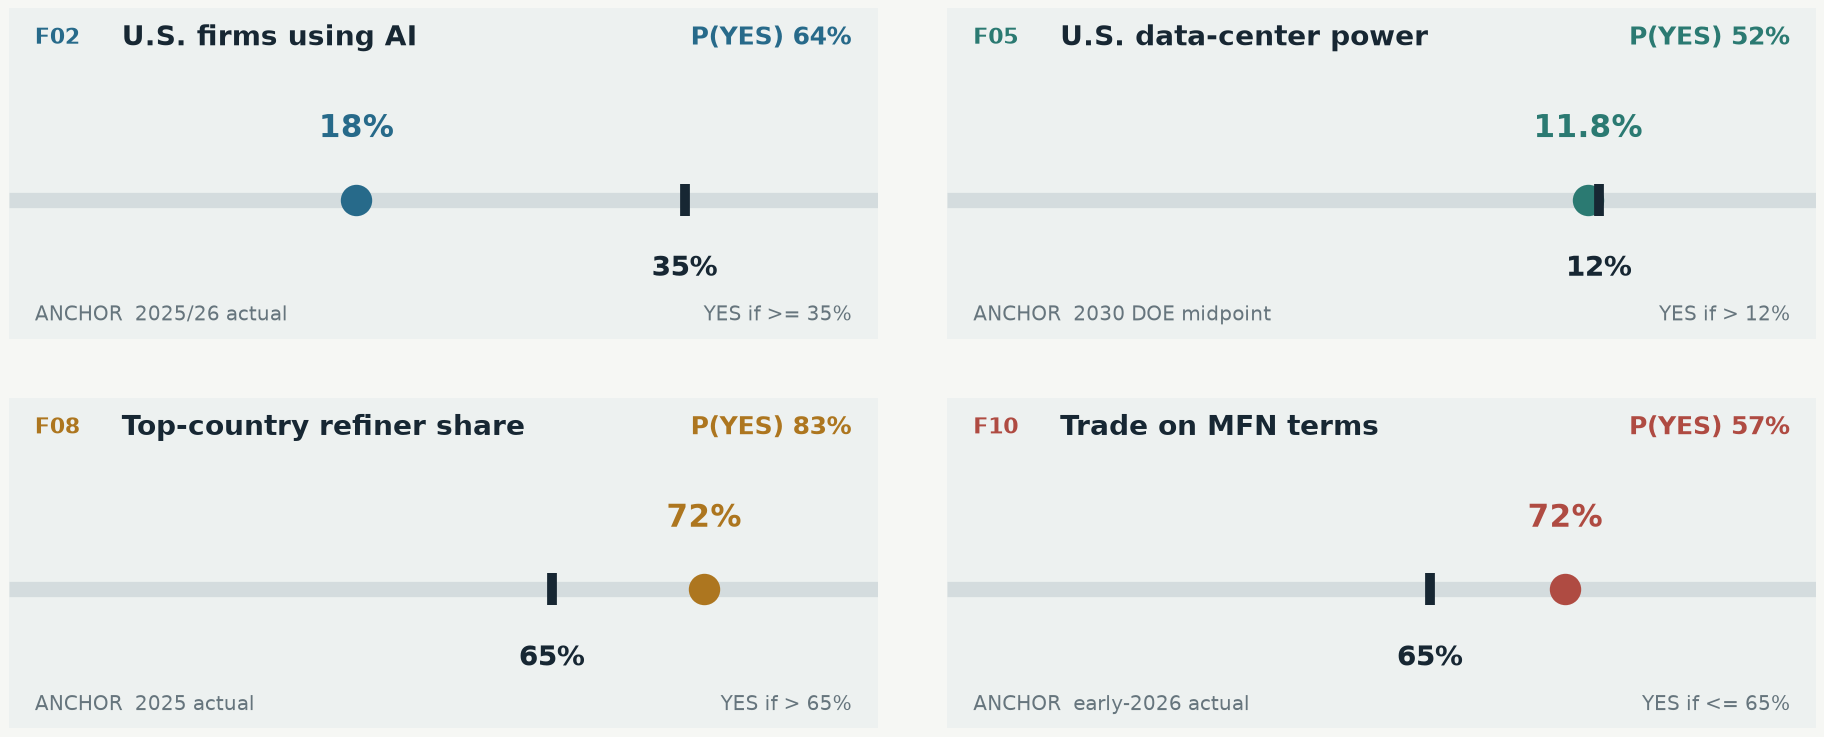
\includegraphics[width=\textwidth]{generated/evidence_dashboard.png}
\end{center}
\vspace{-3pt}
{\scriptsize\color{muted}
\textbf{Four anchors, not four extrapolations.} U.S. firm AI use is
firm-count weighted; the DOE number is its 2030 central estimate; the refining
average excludes rare earths; the MFN share is the WTO's early-2026 estimate.
\src{8,14,19,20}}

\newpage

% PAGE 3 ---------------------------------------------------------------------
\eyebrow{Part 2 --- Framework \& Holistic Synthesis}

\pagetitle{Intelligence gets cheaper; assurance gets dearer}
\vspace{3pt}

\textbf{Thesis.} My highest-conviction claim is not that AI makes everything
scarce. It is that AI changes which scarcities are worth insuring. Cognition is
becoming abundant faster than economies can make power, chips, minerals, data,
capital, and industrial know-how abundant. Modern Mercantilism is the political
response to that mismatch: states pay a premium to secure those complements
inside trusted jurisdictions. The result is an \textit{assured-access economy}.
It fragments strategic nodes, not the global network; raises investment before
measured productivity; and rewards control of bottlenecks more reliably than
ownership of any single model.

Bridgewater's starting point is that national security now enters production
functions directly.\src{3,5} My departure is to model ``AI'' and
``mercantilism'' as one coupled system rather than two parallel resource grabs. Cheap
intelligence increases the value of scarce physical inputs; dependence on
those inputs increases the state's willingness to subsidize and restrict them;
the resulting duplication and cost pressure increase demand for AI efficiency.
That feedback loop explains why rapid capability progress (F01) can coexist
with only a coin-flip power outcome (F05), delayed aggregate productivity
(F03), and stubborn mineral concentration (F08).

\begin{center}
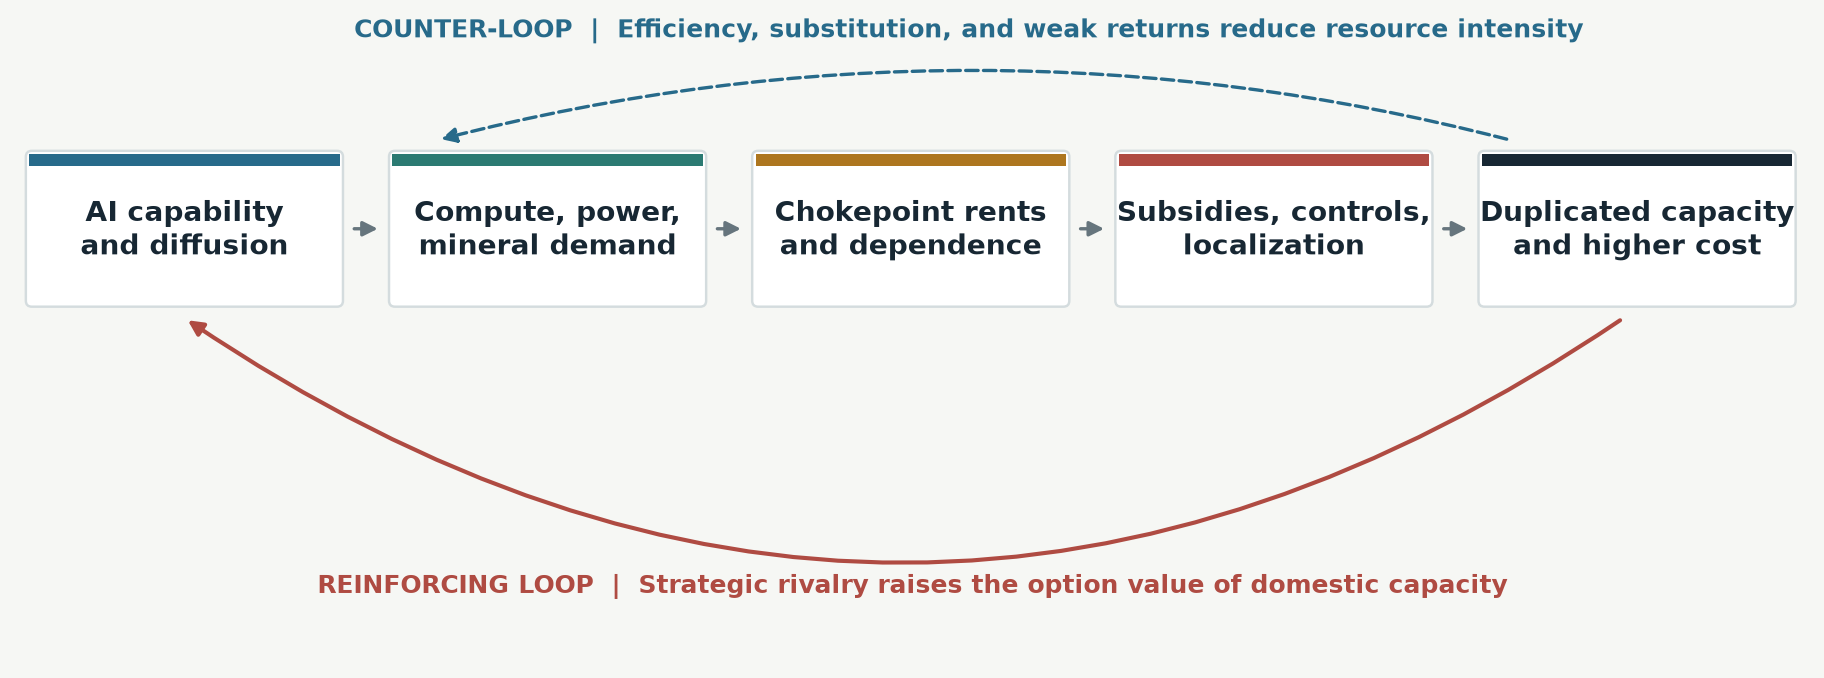
\includegraphics[width=\textwidth]{generated/causal_loop.png}
\end{center}
\vspace{-7pt}

\tighthead{The production function has six serial gates}
Useful AI output is constrained by the weakest of: \textbf{algorithms},
\textbf{accelerators}, \textbf{electricity and grid connection},
\textbf{critical materials}, \textbf{deployable workflows and data}, and
\textbf{political permission}. Substitution exists within a gate, but not
across all gates at once. A better model cannot energize a delayed substation;
a domestic fab cannot operate without tools and skilled technicians; a
national champion cannot create firm-level adoption by decree.

This ``minimum of complements'' structure matters more than heroic estimates
of model intelligence. METR's measured task horizon has risen rapidly, but its
own work warns that long-horizon external validity is uncertain.\src{7}
Conversely, AI output adjusted for falling quality-equivalent prices may be
growing orders of magnitude faster than nominal spending.\src{12} F01 therefore
gets 75\%, not 95\%: the trend is powerful, the measurement bridge is weak.

\tighthead{The timing wedge}
Capability is a laboratory variable; productivity is an organizational
variable. Firms must redesign processes, assign liability, clean data, train
people, and retire old capital. Firm-level cloud evidence finds that learning
continues for roughly four years, while current AI surveys still find perceived
gains ahead of measured gains.\src{11,29} Hence the package predicts fast capability and adoption (F01--F02),
very large capital formation (F04), but only a 46\% chance of productivity
growth clearing 2.25\% through 2030 (F03).

\newpage

% PAGE 4 ---------------------------------------------------------------------
\eyebrow{Part 2 --- Framework \& Holistic Synthesis}

\pagetitle{From comparative advantage to assured access}

\tighthead{1. States target chokepoints, not autarky}
Complete self-sufficiency is arithmetically implausible and economically
wasteful. Policy therefore concentrates on components with high downstream
value, low substitutability, and few suppliers: advanced logic, grid equipment,
magnet materials, cloud capacity, and defense-relevant software. The IEA
estimates that full rare-earth controls could put \$6.5 trillion of annual
downstream production outside China at risk, while the minerals themselves are
a tiny share of final product value.\src{19} That asymmetry makes intervention
rational even when local production costs more.

The result is not classic deglobalization. It is \textbf{rerouting plus
redundancy}: trade remains large, but origin, ownership, and legal jurisdiction
carry an insurance price. U.S. imports from China fell sharply while total U.S.
imports kept growing and activity shifted to established partners such as
Mexico and Vietnam.\src{21} F09 says China's surplus persists because Chinese
firms can redirect exports faster than deficit economies can build complete
supply ecosystems. F10 says discriminatory and preferential lanes keep
expanding, but not that trade collapses.

\vfill
\tighthead{2. Trade balances and capital balances are the same transaction}
The mercantilist ambition to shrink a trade deficit also shrinks the matching
capital inflow. Nir Bar Dea's observation is operationally important: foreign
surpluses helped finance U.S. assets, including the AI build-out; a world that
spends more at home on defense, energy, and compute sends less marginal capital
to U.S. financial markets.\src{28} This does not end U.S. leadership. It changes
its price. The U.S. retains deep capital markets, frontier software, abundant
energy options, and hyperscaler demand; allies acquire more local
infrastructure, while paying higher financing and duplication costs.

\vfill
\tighthead{3. Industrial policy buys capacity more readily than capability}
Subsidies can move factories, especially where scale economies are strong, but
local-content rules also raise cost and can undo much of the demand stimulus.
\src{26} Execution requires utilities, permitting, equipment, skills, customers,
and operating discipline. This distinction separates F06 from F07. Three
advanced-node operators in the U.S. by 2030 receive 78\% because Intel is
already ramping 18A and Samsung and TSMC have funded U.S. paths. Four externally
usable EU gigafactories by 2029 receive only 39\% because the program targets at
most five and construction begins from 2027.\src{16,17,18}

\vfill
\tighthead{4. The AI capex boom is simultaneously demand and supply policy}
Hyperscaler capex supports near-term growth before the systems prove their
revenue yield. Bridgewater estimates a large 2026--27 U.S. growth contribution,
but notes that the build is labor-light and can crowd out other investment.
\src{4} Competition turns underinvestment into the career and national-security
risk, so spending can overshoot private return. That makes F04 more likely than
F03. It also creates the key downside: if inference demand or monetization
disappoints, cancellations propagate through power, chips, and construction
well before software capability reverses.

\vfill
\begingroup
\renewcommand{\arraystretch}{1.42}
\begin{tabularx}{\textwidth}{@{}>{\sffamily\bfseries}p{0.19\textwidth}X>{\sffamily\bfseries}p{0.19\textwidth}X@{}}
\color{blue}Scales quickly & software capability, model access, trade rerouting &
\color{ink}Scales slowly & grids, refineries, skills, institutions\\
\color{red}Policy can buy & redundant plant, inventory, demand guarantees &
\color{ink}Policy cannot buy & tacit know-how, utilization, trust, productivity\\
\end{tabularx}
\endgroup

\newpage

% PAGE 5 ---------------------------------------------------------------------
\eyebrow{Part 2 --- Framework \& Holistic Synthesis}

\pagetitle{Distribution, scenarios, and falsification}

\tighthead{Who wins}
\begin{itemize}
  \item \textbf{Owners of scarce complements:} power developers, grid and
  cooling suppliers, advanced foundries, semiconductor equipment firms, and
  refiners with secure feedstock. They earn scarcity rents even when model
  margins compress.
  \item \textbf{The U.S. stack, conditionally:} software, capital markets,
  hyperscaler balance sheets, and energy depth reinforce one another. F04--F06
  embody that advantage, but high asset prices and capital diversion reduce
  investor returns relative to real capacity growth.
  \item \textbf{China's manufacturing ecosystem:} export destinations change,
  yet supplier density, infrastructure, and cost advantages persist. China can
  lose U.S. share while sustaining a trillion-dollar surplus (F09).
  \item \textbf{Power-rich and resource-rich middle powers:} countries that
  offer reliable energy, minerals, permitting, and geopolitical optionality
  gain bargaining power as firms pay for jurisdictional diversification.
\end{itemize}

\tighthead{Who loses}
\begin{itemize}
  \item \textbf{Energy-poor industrial importers} pay three premiums at once:
  expensive power, duplicated capacity, and mineral security.
  \item \textbf{Routine entry-level cognitive labor} faces a flow problem
  before an aggregate unemployment shock: fewer openings, weaker training
  ladders, and gains captured by capital and complementary experts. Current
  evidence shows exposure and slower young-worker hiring, not yet mass
  displacement.\src{10}
  \item \textbf{Consumers and taxpayers in bottleneck jurisdictions} fund
  subsidies and bear tariff incidence. Protection can create capacity while
  lowering real income; those statements are not contradictory.
  \item \textbf{Universal institutions} lose authority to bilateral bargains,
  clubs, and interim workarounds. F11 is the institutional counterpart to F10
  and F12.
\end{itemize}

\tighthead{Three coherent worlds}
\begin{tabularx}{\textwidth}{@{}>{\bfseries}p{0.18\textwidth}>{\centering\arraybackslash}p{0.08\textwidth}X@{}}
\toprule
Scenario & Weight & Joint implications\\
\midrule
\color{blue}Abundant AI & 25\% & Week-scale agents arrive early;
diffusion and productivity accelerate; efficiency softens physical scarcity
and trade discrimination is less necessary.\\
\color{red}Bottlenecked boom & 50\% & Capability and capex stay fast, but power,
materials, implementation, and national rivalry bind; real productivity trails
nominal investment. This is the modal world.\\
\color{gold}Retrenchment & 25\% & Returns disappoint and AI construction
slows; strategic rivalry, tariffs, mineral concentration, and institutional
paralysis persist because their political causes predate the boom.\\
\bottomrule
\end{tabularx}

\tighthead{The decisive asymmetry}
AI forecasts fall sharply in the retrenchment world; mercantilism forecasts do
not. That is deliberate. Modern Mercantilism is not merely an AI investment
cycle: it is rooted in security competition, domestic distribution, and the
failure of prior rules to discipline non-market policy. AI intensifies the
competition but need not cause it.

\tighthead{Kill criteria}
The framework is wrong if three developments occur together by 2028:
quality-adjusted inference becomes radically less resource-intensive,
hyperscalers cut real capex without a demand rebound, and major states restore
non-discriminatory trade rather than redirect restrictions through narrower
instruments. It is also wrong if subsidized capacity achieves incumbent-level
utilization and cost quickly. Those outcomes would break the bottleneck loop,
raise F03, and lower F04--F05 and F08--F12 together. A framework that cannot
lose as a bundle is only a story.

\newpage

% PAGE 6 ---------------------------------------------------------------------
\eyebrow{Part 3 --- Analytical Appendix}

\pagetitle{Method: calibrated judgment under shared shocks}

\tighthead{Evidence hierarchy}
I used official realized data and contractual resolution sources first; audited
company disclosures second; peer-reviewed or high-quality working papers
third; and interviews only as management/policy signals. Vendor claims were
never treated as base rates. Every forecast was tested through four lenses:
historical prior, current trend, policy execution, and the strongest plausible
countercase. Their robust log-odds center is a diagnostic anchor, not a second
probability engine. I then specified conditionals inside three coherent macro
worlds so that one forecast could not quietly assume a boom while another
assumed a bust. This borrows the useful search--reconcile--calibrate discipline
from Bridgewater AIA Labs without pretending that twelve bespoke questions
form a statistical calibration sample.\src{6}

\begin{center}
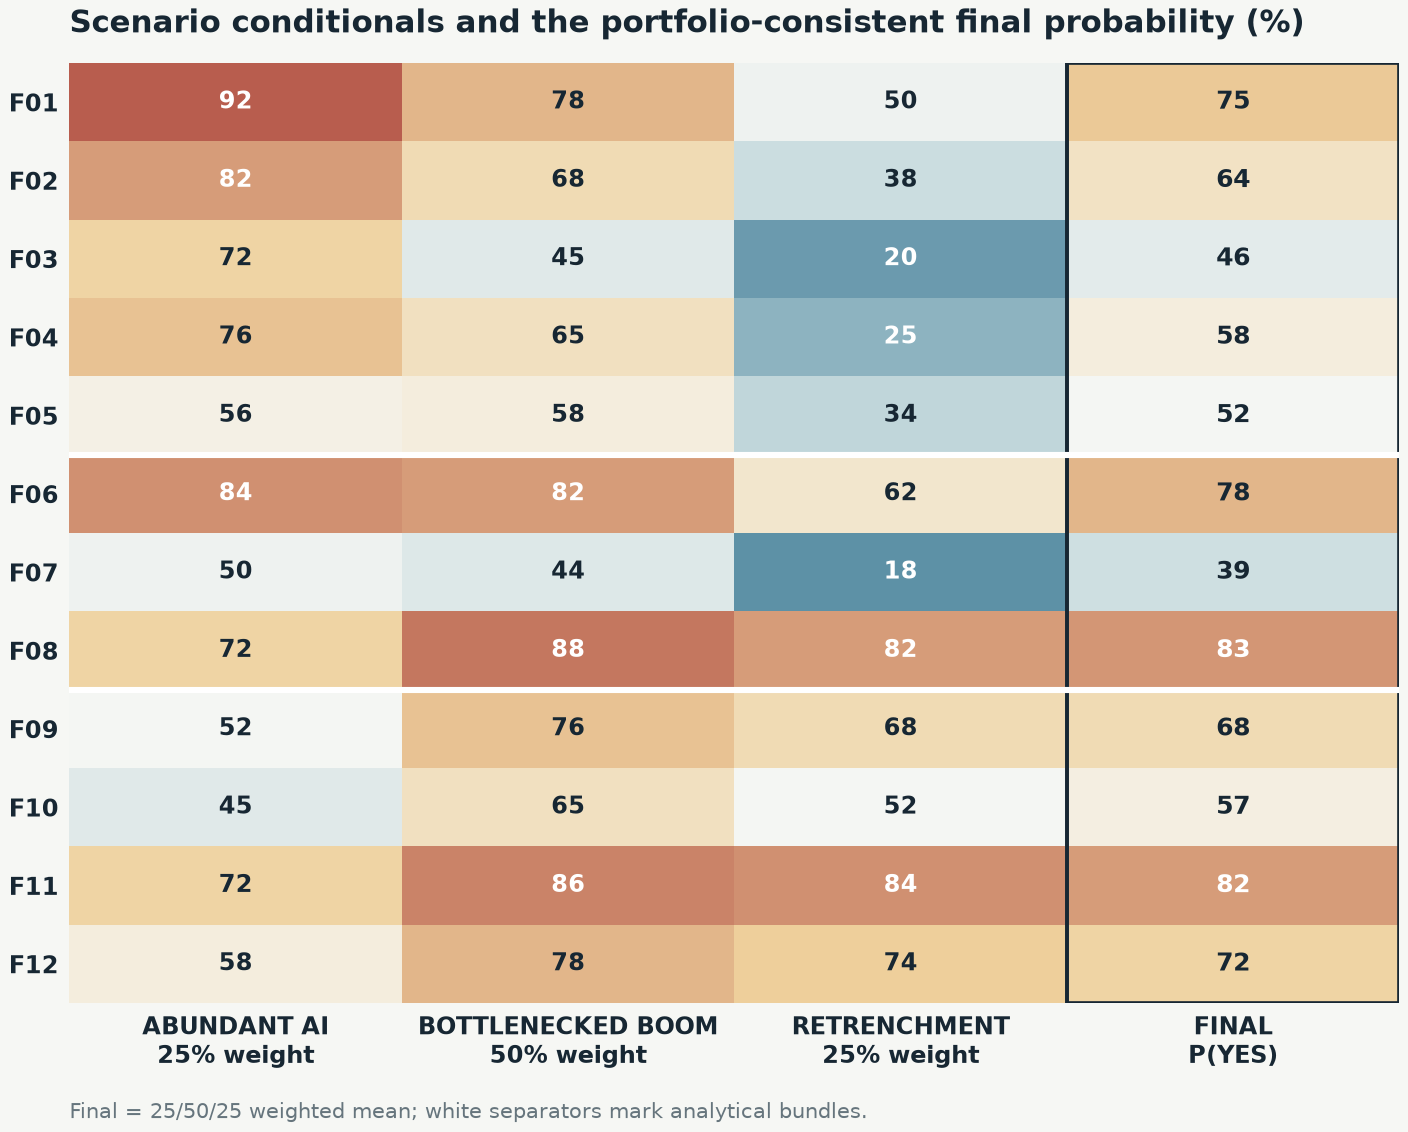
\includegraphics[height=4.05in]{generated/scenario_heatmap.png}
\end{center}
\vspace{-7pt}

The outlined final column is the 25/50/25 scenario-weighted mean, rounded to
the nearest point. It remains close to the independent lens anchor for every
forecast; the largest gap is six points. Conditionals are judgments, not fitted
likelihoods. Transparent structure is preferable to fake precision.

\tighthead{Correlation map and scoring discipline}
\begin{tabularx}{\textwidth}{@{}>{\bfseries}p{0.21\textwidth}p{0.18\textwidth}X@{}}
\toprule
Bundle & Forecasts & Shared shock\\
\midrule
AI scale & F01, F02, F04, F05 & capability demand, monetization, efficiency,
grid execution\\
AI macro & F02, F03, F04 & organizational diffusion versus crowding out and
measurement lag\\
Industrial policy & F06, F07, F08 & subsidy persistence, permitting, skills,
equipment, cost gap\\
Trade regime & F09--F12 & U.S.-China policy, retaliation, rerouting, WTO
institutional repair\\
\bottomrule
\end{tabularx}

The forecasts should not be read as twelve independent bets. Under a capex
bust, F01--F05 tend to resolve lower together. Under a durable U.S.-China
settlement, F09--F12 tend to resolve lower together. I avoided extremizing
those clusters because correlated evidence creates less independent
information than twelve separate headlines suggest.

\newpage

% PAGE 7 ---------------------------------------------------------------------
\eyebrow{Part 3 --- Analytical Appendix}

\pagetitle{AI: capability outruns diffusion; diffusion outruns GDP}

\tighthead{F01 --- One-week task horizon (75\%)}
METR's fitted trends have historically doubled the 50\% task horizon in roughly
four to seven months, putting a one-week threshold inside 2029 under substantial slowdown.
The upward case is reinforced by test-time compute, tool use, memory, and
agent scaffolding. The discount is severe because current suites contain few
tasks beyond roughly 16 human hours, scoring long autonomous chains is hard,
and software benchmarks may not transfer to open-ended economic work.
\src{7} \textbf{Sensitivity:} roughly $-15$ points if the measured doubling
time exceeds one year through 2027; $+10$ if an independent suite validates a
48-hour horizon by end-2027.

\vfill
\tighthead{F02 --- 35\% of firms using AI (64\%)}
The redesigned Census question is broad but the denominator is demanding:
18\% of firms used AI in a business function in late 2025/early 2026, versus
32\% when weighted by employment; only 22\% expected use within six months.
\src{8} Adoption is concentrated in large knowledge firms, so enterprise
headlines overstate the count-weighted base. Falling prices and embedded
software support an S-curve; data, liability, and weak small-firm complements
slow it. \textbf{Sensitivity:} $-12$ if BTOS remains below 23\% at end-2027;
$+10$ if it clears 27\%.

\vfill
\tighthead{F03 --- Productivity above 2.25\% (46\%)}
Task-level gains can be large, but aggregation multiplies them by adoption,
task coverage, and reorganization. Recent executive surveys find little
realized firm impact, expected gains around 1.4\% over three years, and a gap
between perceived and measured productivity.\src{11} The upside is that
quality-adjusted AI output and usage value are already large and poorly
captured in prices.\src{12} The downside is crowding out, transition costs, and
labor-light capex. \textbf{Sensitivity:} F03 rises above 60\% only if both F02
and broad workflow redesign accelerate by 2028.

\vfill
\tighthead{F04 --- \$1 trillion of four-firm capex (58\%)}
The threshold requires high-teens annual growth from an already extraordinary
2026 run rate. Demand visibility, competitive fear, and sovereign customers
support it; power availability, depreciation, financing needs, and weak
inference revenue oppose it. Executives and chip suppliers are informative
about orders but structurally bullish, so their ``no bust'' claims receive low
weight.\src{5,13,28} \textbf{Sensitivity:} $+12$ if the four companies' 2027
guidance exceeds \$850 billion; $-20$ if two cut planned AI capacity.

\vfill
\tighthead{F05 --- Data centers above 12\% of U.S. power (52\%)}
DOE/LBNL's 2030 central estimate is 11.8\%, with a 9.5--15.3\% range.\src{14}
The forecast sits just above the midpoint on purpose: capex evidence has moved
up, but grid interconnection, transformer supply, local opposition, utilization,
and efficiency can ration consumption. The IEA estimates that delayed grid
connections put around one-fifth of planned projects at risk.\src{15}
Efficiency lowers joules per token yet can raise total use through cheaper
inference; the net sign is genuinely close.

\newpage

% PAGE 8 ---------------------------------------------------------------------
\eyebrow{Part 3 --- Analytical Appendix}

\pagetitle{The physical stack: capacity is not sovereignty}

\tighthead{F06 --- Three U.S. advanced-node operators (78\%)}
This is a count of corporate operators, not fabs. Intel reported 18A in
high-volume production; Samsung targets 2nm at Taylor; TSMC's Arizona sequence
includes 2nm-or-better capacity. Commerce expects the U.S. leading-edge logic
share to rise from zero in 2022 to about 20\% in 2030.\src{16,17} The main
failure modes are yield, customer qualification, equipment timing, and
megaproject delay: Intel pushed Ohio operations to 2030--31. The threshold
therefore demands commercial production but not cost parity or a large global
share. \textbf{Sensitivity:} $-18$ if Samsung Taylor has not begun commercial
production by end-2027.

\vfill
\tighthead{F07 --- Four operational EU gigafactories (39\%)}
The EU has demonstrated that it can launch smaller AI Factories, but the
gigafactory target is up to five, with roughly EUR20 billion to mobilize and
first construction scheduled from 2027.\src{18} Four facilities serving
outside users within three years leaves little tolerance for procurement,
financing, grid, chip, or commissioning delays. Counting announcements would
confuse fiscal intent with compute service. The low probability is not a claim
that Europe builds nothing; two or three operational sites would still be a
major strategic shift. \textbf{Sensitivity:} $+20$ if four projects reach
financial close and energization contracts by mid-2027.

\vfill
\tighthead{F08 --- Refining concentration above 65\% (83\%)}
The average leading-country share across the fixed six-mineral basket was about
72\% in 2025 excluding rare earths, up from 70\% in 2023.\src{19} Announced
diversification is skewed upstream: refining projects outside incumbents face
20--150\% higher capital costs, roughly 50\% higher operating costs, specialized
equipment gaps, and slow disbursement of public finance. AI and grid build-outs
raise demand for copper, graphite, and related materials while export controls
increase the option value of incumbent capacity. A seven-point decline is
possible, but it requires several projects to operate, not merely close
financing. \textbf{Sensitivity:} $-15$ if the same-basket average is below 68\%
in the IEA's 2028 report.

\vfill
\tighthead{Why the three forecasts do not conflict}
F06 predicts geographic duplication in the highest-value semiconductor stage.
F08 predicts persistence of concentration deeper in the material stack. Both
can be true because states can subsidize a handful of \$20 billion fabs more
readily than reproduce every refinery, equipment vendor, supplier network, and
skill base feeding them. F07 is lower because Europe is attempting several
gates simultaneously while starting from a compute and energy disadvantage.

\vfill
\begingroup
\renewcommand{\arraystretch}{1.25}
\begin{tabularx}{\textwidth}{@{}>{\sffamily\bfseries}p{0.20\textwidth}XXX@{}}
\toprule
Test & \textbf{F06 U.S. fabs} & \textbf{F07 EU compute} & \textbf{F08 minerals}\\
\midrule
Money committed & strong & meaningful & rising\\
Execution chain & medium & long & very long\\
Incumbent cost gap & manageable & material & often extreme\\
Resolution requires & production & external workloads & global share loss\\
\bottomrule
\end{tabularx}
\endgroup

\newpage

% PAGE 9 ---------------------------------------------------------------------
\eyebrow{Part 3 --- Analytical Appendix}

\pagetitle{Trade: rerouting is not rebalancing}

\tighthead{F09 --- China's trillion-dollar surplus twice (68\%)}
China's 2025 goods surplus was roughly \$1.2 trillion. Industrial depth, weak
domestic absorption, and rapid destination switching support persistence;
U.S. import decoupling alone does not erase the global surplus. Federal Reserve
work attributes China's export strength partly to industrial policy, while the
IMF's countercase is explicit: stronger consumption, property repair, exchange
rate adjustment, and partner restrictions could compress external imbalance.
\src{22,23} Requiring two years, not one, protects against commodity and FX
noise. \textbf{Sensitivity:} $-15$ if China's 2027 surplus is below \$800
billion alongside a rising household-consumption share.

\vfill
\tighthead{F10 --- MFN trade share at or below 65\% (57\%)}
The WTO estimates that MFN treatment covered 80\% of merchandise trade in 2024
but about 72\% by early 2026. The decline mixes punitive tariffs with
preferential agreements, exactly the movement from universal rules to trusted
lanes.\src{20} Reaching 65\% requires another material shift; exemptions and
supply-chain adaptation could stabilize the share. AI-enabling goods are a
counterforce: they represented one-sixth of trade but 42\% of 2025 trade growth
and were often exempt from new tariffs. This is why F10 is 57\%, not a
straight-line 80\%.

\vfill
\tighthead{F11 --- Appellate Body still below quorum (82\%)}
The body has been unable to hear new appeals since December 2019. Interim
arbitration can reduce pressure to solve the underlying appointment dispute,
and broader trade conflict makes a consensus bargain harder. A reform package
remains possible, so the probability stops well below certainty. The exact
roster makes this the cleanest institutional forecast: alternative mechanisms
do not count. \textbf{Sensitivity:} $-25$ on a U.S.-backed appointments
agreement with implementation dates before 2029.

\vfill
\tighthead{F12 --- U.S. effective tariff at least 8\% (72\%)}
The relevant rate is cash duties divided by customs value, not an announced
headline. The 2026 policy baseline is already above the pre-2025 norm, and
tariff revenue, bargaining leverage, and industrial goals create persistence
across legal forms.\src{24} Offsetting forces are court decisions, exemptions,
trade deals, substitution toward low-duty suppliers, and domestic incidence.
Historical evidence finds rapid import contraction and substantial importer
burden after large tariffs; economic cost does not guarantee political
reversal.\src{27}

\vfill
\begin{center}
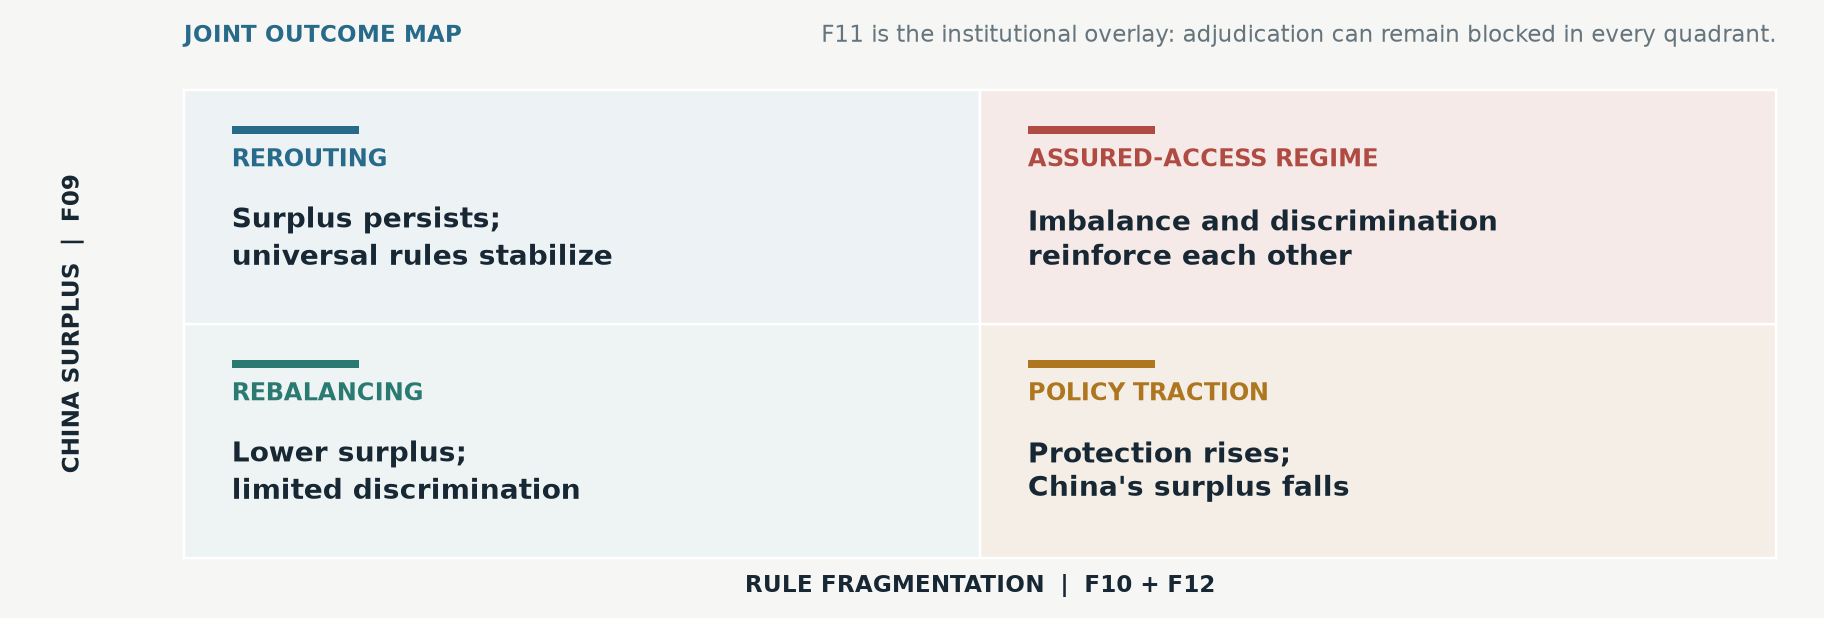
\includegraphics[width=\textwidth]{generated/trade_matrix.png}
\end{center}

\newpage

% PAGE 10 --------------------------------------------------------------------
\eyebrow{Resolution Registry and Selected Sources}

\pagetitle{Resolve the words, not the narrative}
\vspace{2pt}

{\fontsize{8.0}{9.3}\selectfont
\begin{multicols}{2}
\raggedcolumns

\textbf{\color{blue}Resolution protocol.} Equality follows the sentence
(``at least'' includes it; ``more than'' does not). Use the first qualifying
official release by June 30, 2031 and its then-current vintage unless a
forecast below specifies another date. Later revisions do not reopen a result.
A documented comparable successor series is allowed; otherwise the stated
fallback applies or the event resolves No.

\textbf{F01} System generally available by 2029-12-31; METR must publish by
2030-06-30 a non-saturated-suite 50\% point estimate $\geq168$ hours. No
documented successor: No.

\textbf{F02} National firm-count-weighted core BTOS answer to AI use in any
business function during the prior two weeks, collection period ending latest
in 2028; original release.

\textbf{F03} From the BLS release available 2031-06-30, compute
$(LP_{2030Q4}/LP_{2026Q4})^{1/4}-1$; Yes only if $>2.25\%$.

\textbf{F04} Sum 2028 calendar-quarter company-disclosed capex excluding
acquisitions, using restated comparable definitions; Amazon includes equipment
acquired under finance leases and Microsoft is calendar-aligned.

\textbf{F05} First DOE/LBNL study by 2032-12-31 estimating actual 2030 data
center and total U.S. electricity; EIA fallback; neither reports both: No.

\textbf{F06} Count corporate operators, not fabs; operator-filed commercial
high-volume/mass wafer production at a U.S. fab. Marketed node names apply
(Intel 18A qualifies); risk production and packaging do not.

\textbf{F07} EU location, formal InvestAI/EuroHPC gigafactory selection, and at
least one accepted allocation from a legally separate external user by
2029-12-31. AI Factories/antennas do not count.

\textbf{F08} Unweighted mean of the top refiner's 2030 share for copper,
lithium, nickel, cobalt, graphite, and manganese in the first IEA report by
2032-06-30. One missing: use five; two missing: No.

\textbf{F09} GACC annual U.S.-dollar goods exports minus imports; at least two
of 2027--29 must each be strictly above \$1 trillion.

\textbf{F10} WTO 2029 year-end MFN merchandise-trade share first published by
2030-06-30; use midpoint of a range; no comparable update: No.

\textbf{F11} WTO Appellate Body roster at 23:59 UTC on 2029-12-31; fewer than
three members is Yes regardless of interim arbitration.

\textbf{F12} For each year divide duties collected by customs value for total
imports in USITC DataWeb; arithmetic mean of 2027--29 rates from data
downloaded 2030-06-30; Yes at $\geq8.000\%$.

\columnbreak

\textbf{\color{blue}Selected sources.}

\textbf{[1]} Bridgewater/Global Citizen, \href{https://observatory.bwater.com/events/2026-forecasting-the-future}{Forecasting the Future 2026 brief}, accessed Jul.\ 30, 2026.

\textbf{[2]} Bridgewater/Global Citizen, \href{https://www.bridgewater.com/bridgewater-global-citizen-forecasting-the-future-a-modern-economics-challenge-2026-terms-conditions}{Terms and Conditions}, 2026.

\textbf{[3]} Bridgewater, \href{https://www.bridgewater.com/research-and-insights/were-all-mercantilists-now}{We're All Mercantilists Now}, 2024.

\textbf{[4]} Bridgewater, \href{https://www.bridgewater.com/research-and-insights/the-macro-implications-of-the-ai-capex-boom}{The Macro Implications of the AI Capex Boom}, Jan.\ 2026.

\textbf{[5]} Bridgewater, \href{https://www.bridgewater.com/the-accelerating-resource-grabs-in-ai-and-modern-mercantilism-content-ctd}{The Accelerating Resource Grabs in AI and Modern Mercantilism}, Apr.\ 2026.

\textbf{[6]} Bridgewater AIA Labs, \href{https://arxiv.org/abs/2511.07678}{AIA Forecaster Technical Report}, 2025.

\textbf{[7]} METR, \href{https://metr.org/time-horizons/}{Task-Completion Time Horizons} and 2026 measurement-limitations notes.

\textbf{[8]} Bonney et al., \href{https://www.nber.org/papers/w35141}{The Microstructure of AI Diffusion}, NBER 35141, 2026; U.S. Census BTOS.

\textbf{[9]} Stanford HAI, \href{https://hai.stanford.edu/ai-index/2026-ai-index-report}{AI Index Report 2026}.

\textbf{[10]} Anthropic, \href{https://www.anthropic.com/research/labor-market-impacts}{Labor Market Impacts of AI}, 2026; Stanford Digital Economy Lab, AI Economic Indicators, 2026.

\textbf{[11]} Yotzov et al., \href{https://www.nber.org/papers/w34836}{Firm Data on AI}, NBER 34836, 2026; Baslandze et al., NBER 34984, 2026.

\textbf{[12]} Korinek and McKelvey, \href{https://papers.ssrn.com/sol3/papers.cfm?abstract_id=6813982}{Measuring the AI Economy}, 2026; Fan and Nguyen, IMF WP 26/147.

\textbf{[13]} Alphabet, Amazon, Meta, and Microsoft filings and earnings calls through Jul.\ 30, 2026.

\textbf{[14]} DOE/LBNL, \href{https://www.energy.gov/powering-americas-ai-future-data-center-resource-hub}{U.S. Data Center Energy Usage Report 2025 Update}.

\textbf{[15]} IEA, \href{https://www.iea.org/reports/key-questions-on-energy-and-ai/executive-summary}{Key Questions on Energy and AI}, 2026.

\textbf{[16]} U.S. GAO, \href{https://www.gao.gov/products/gao-26-107882}{Semiconductor Projects}, GAO-26-107882.

\textbf{[17]} Intel, Samsung, and TSMC official production disclosures through Jul.\ 30, 2026.

\textbf{[18]} European Commission, \href{https://commission.europa.eu/topics/competitiveness/competitiveness-coordination-tool-projects/ai-gigafactories_en}{AI Gigafactories}, accessed Jul.\ 30, 2026.

\textbf{[19]} IEA, \href{https://www.iea.org/reports/global-critical-minerals-outlook-2026/executive-summary}{Global Critical Minerals Outlook 2026}.

\textbf{[20]} WTO, \href{https://www.wto.org/english/news_e/news26_e/stat_19mar26_329_e.htm}{Global Trade Outlook and Statistics}, Mar.\ 2026; \href{https://data.wto.org/en/dataset/mfnshare}{MFN trade-share dataset}.

\textbf{[21]} Alfaro and Chor, \href{https://www.nber.org/papers/w34490}{An Anatomy of the Great Reallocation}, NBER 34490, 2025/26.

\textbf{[22]} Federal Reserve Board, \href{https://www.federalreserve.gov/econres/notes/feds-notes/chinas-trade-dominance-and-the-role-of-industrial-policies-20260323.html}{China's Trade Dominance}, Mar.\ 2026.

\textbf{[23]} IMF, \href{https://www.imf.org/-/media/files/publications/cr/2026/english/1chnea2026001-source-pdf.pdf}{China 2025 Article IV}, 2026.

\textbf{[24]} USITC \href{https://dataweb.usitc.gov/}{DataWeb}; WTO--IMF Tariff Tracker; Yale Budget Lab, State of U.S. Tariffs, Apr.\ 2026.

\textbf{[25]} WTO, Appellate Body \href{https://www.wto.org/english/tratop_e/dispu_e/ab_members_descrp_e.htm}{member roster}, accessed Jul.\ 30, 2026.

\textbf{[26]} Head et al., \href{https://www.nber.org/papers/w34884}{Industrial Policies for Multi-Stage Production}, NBER 34884, 2026.

\textbf{[27]} Mitchener and Pedemonte, \href{https://www.nber.org/papers/w35249}{The Price of Protection}, NBER 35249, 2026.

\textbf{[28]} Nir Bar Dea, Unholy podcast, Jun.\ 2026; Greg Jensen, Bridgewater Daily Observations, 2026; Jensen Huang and Dario Amodei interviews, used only as directional signals.

\textbf{[29]} Brand et al., \href{https://www.nber.org/papers/w32938}{Firm Productivity and Learning with Digital Technologies}, NBER 32938, rev.\ 2025.

\vfill
\textbf{\color{red}Draft governance note.} The entrant must independently
challenge and approve the thesis, wording, probabilities, and prose before
submission under the competition's authorship terms.\src{2}

\end{multicols}
}

\end{document}
